% problems.tex

\begin{frame}
    \frametitle{Fixing the leaks}

    \notes{If we claim it is not capable of independent computation, then we don't make it do independent computation}

    \begin{center}
        \emph{\textcolor{Periwinkle}{Use as a subroutine!}}
    \end{center}

    % add VQA tradeoff diagram
    \begin{center}
        \vspace{1em}
        \begin{figure}
            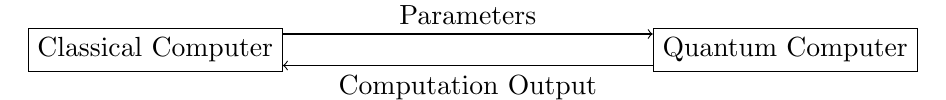
\begin{tikzpicture}[node distance = 8cm]
                \node[draw, rectangle] (C) {Classical Computer};
                \node[draw, rectangle, right of=C] (Q) {Quantum Computer};
	
                
                \begin{scope}[transform canvas={yshift=0.2cm}]
                    \draw[->] (C) -- node[above, midway] {Parameters} (Q);
                \end{scope}
                
                \begin{scope}[transform canvas={yshift=-0.2cm}]
                    \draw[->] (Q) -- node[below, midway] {Computation Output} (C);
                \end{scope}
            \end{tikzpicture}
        \end{figure}
        \vspace{1em}
    \end{center}

\end{frame}

\begin{frame}
    \frametitle{Quantum Bandaid}

    Tides us over while people look for exotic materials and configurations to
    attain reasonable coherence!

    \begin{itemize}
        \item[\textcolor{OliveGreen}{\checkmark}] Computational efficiency of a quantum computer
        \item[\textcolor{OliveGreen}{\checkmark}] Control efficiency of a classical system
        \item[\textcolor{OliveGreen}{\checkmark}] Allows alternate explorations for quantum supremacy
    \end{itemize}

\end{frame}

\begin{frame}
    \frametitle{A Solution}

    \begin{center}
        \textcolor{Periwinkle}{\large Variational Quantum Algorithms \footfullcite{cerezo2021vqa}}

        \begin{figure}
            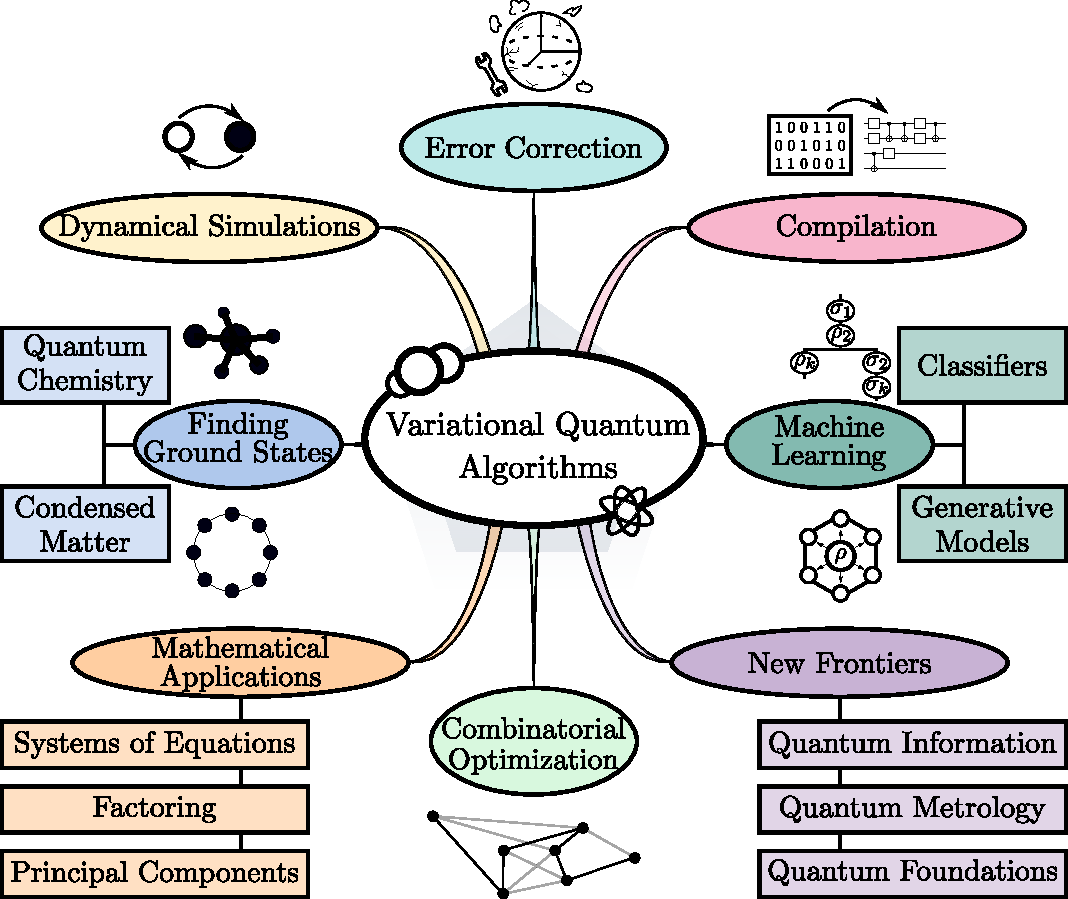
\includegraphics[width=0.4\textwidth]{figures/vqaapp.pdf}
        \end{figure}
    \end{center}

\end{frame}